\documentclass[10pt,a4paper]{article}
\usepackage[utf8]{inputenc}
\usepackage[T1]{fontenc}
\usepackage{lmodern}
\usepackage[english]{babel}
\usepackage[margin=2.0cm]{geometry}
\usepackage{amsmath,amssymb,mathtools,bm}
\usepackage{booktabs,array,tabularx,longtable}
\newcolumntype{L}[1]{>{\raggedright\arraybackslash}p{#1}}
\newcolumntype{Y}{>{\raggedright\arraybackslash}X}
\usepackage{graphicx}
\usepackage{float}
\usepackage[font=small]{caption}
\usepackage{xcolor}
\usepackage{tikz}
\usetikzlibrary{arrows.meta,positioning,decorations.pathmorphing,decorations.pathreplacing,patterns,calc}
\usepackage[hidelinks]{hyperref}
\usepackage{url}
\makeatletter\g@addto@macro{\UrlBreaks}{\do\_\do/}\makeatother
\numberwithin{equation}{section}
\setlength{\emergencystretch}{3em}
\newcommand{\note}[1]{\begin{center}\fcolorbox{red!70!black}{red!5}{\parbox{0.94\linewidth}{\small\textbf{Note.} #1}}\end{center}}
\input{generated/numbers}

\tikzset{
  mass/.style={draw, thick, fill=gray!8, minimum width=1.45cm, minimum height=0.95cm, align=center, font=\small},
  spring/.style={decorate, decoration={zigzag, pre length=2.5mm, post length=2.5mm, segment length=5pt, amplitude=3pt}},
  lab/.style={font=\scriptsize, inner sep=1.5pt},
  sig/.style={-{Latex[length=2mm]}, thick},
  meas/.style={-{Latex[length=2mm]}, dashed, blue!60!black},
  blk/.style={draw, rounded corners, align=center, minimum height=0.9cm, fill=blue!4, font=\small},
}
\newcommand{\ground}[3]{\draw[thick] (#1,#3) -- (#2,#3); \fill[pattern=north east lines] (#1,#3) rectangle (#2,#3-0.18);}

\title{Elevation resonances of the LUCY mount as fork modes driven by the motor stator:\\ a data-driven lumped model with two stator modal masses, and a flexible azimuth load}
\author{Generated by \texttt{build\_fork\_modes\_report.py}\\ \small\texttt{sim/gimbal\_multidof/report\_fork\_modes}}
\date{\today}
\begin{document}
\maketitle

\paragraph{Purpose.} Frequency responses taken with the motion of the fork constrained showed that the resonances of the elevation axis below 150\,Hz are vibrations of the fork, which also explains why resonances at the same frequencies appear on the azimuth axis. This report describes how a data-driven model of those resonances was built and identified:
\begin{itemize}
\item on the elevation axis, the lumped model H7 is extended with \emph{modal masses attached to the motor stator}. The reaction of the motor torque excites them, and they move the encoder read head, which is mounted on the same structure;
\item on the azimuth axis, the load of H7 is split into a fork base and a fork top joined by a spring, so that the load is no longer rigid.
\end{itemize}
The step documented here is the reduced elevation model with \textbf{two} stator masses. Of the four masses of the previous iteration (\massesFour\,Hz), the ones at 8.8 and 53.4\,Hz were removed and the model was refitted. All the results refer to the fit band \textbf{1--150\,Hz}.

\paragraph{Main results.}
\begin{itemize}
\item \textbf{Elevation.} Two stator masses, at \fMassI\,Hz and \fMassII\,Hz, with residues of opposite sign.
  \begin{itemize}
  \item The fit (NRMSE on the complex response, 1--150\,Hz) on the three nominal measurements goes from \fitHPI, \fitHPII\ and \fitHPIII\,\% with H7 to \fitPI, \fitPII\ and \fitPIII\,\%.
  \item The rms errors are 1.7--2.2\,dB in magnitude and 7.6--17.9$^\circ$ in phase.
  \item All \nStartsP\ starts of the least squares end in the same minimum.
  \end{itemize}
\item \textbf{Non-collocated mode.} In the mode at \fMassI\,Hz the encoder head moves against the stator (negative residue).
  \begin{itemize}
  \item With the mode at \fMassII\,Hz, this produces a quartet of zeros, \zerosP: one pair is in the right half-plane.
  \item This pair explains the extra phase drop of about 360$^\circ$ measured between 45 and 120\,Hz.
  \end{itemize}
\item \textbf{Azimuth.} With the flexible load the fit goes from \fitHA\,\% (H7) to \fitA\,\% (\dbA\,dB, \degA$^\circ$ rms).
  \begin{itemize}
  \item The fork mode at \fForkAz\,Hz has the motor and the fork base moving against the fork top and the telescope.
  \item It lies at the frequency of the elevation stator mass at \fMassI\,Hz: the same fork vibration is seen by both axes.
  \end{itemize}
\item \textbf{Cost of the reduction.} Removing the masses at 8.8 and 53.4\,Hz loses the antiresonance--resonance pair at 8--9\,Hz.
  \begin{itemize}
  \item The fit of the 1--600\,Hz measurement between 5 and 100\,Hz drops from 66 to 32\,\%.
  \item Above 30\,Hz the two-mass model is as good as the four-mass one.
  \end{itemize}
\end{itemize}

\note{The H7 configuration contains placeholder data: the inertias of the encoder and motor nodes, the materials, and the elevation during the tests (taken as $\theta_0=0$). The figures therefore carry the label ``result from placeholder parameters''. The inertias are kept fixed at the CAD/H7 values in all the fits.}

\tableofcontents

%% ===================================================================================================
\section{Data}\label{sec:data}
Four frequency responses measured with Kollmorgen WorkBench on 28/10/2026 (folder \path{LucyIdentification/Poli_Polar_identification}), all taken 12\,mm from the end stop (Table~\ref{tab:data}). The measured quantity is the WorkBench trace ``Plant'':
\begin{itemize}
\item the encoder velocity over the commanded current, in (rad/s)/A;
\item measured with a stepped-sine current excitation, an FFT of 4096 points and 50\,\% overlap;
\item smoothed by WorkBench by 1\,\% in frequency.
\end{itemize}
\begin{equation}
G_\mathrm{mis}(j\omega)=\frac{\Omega_\mathrm{enc}(j\omega)}{I(j\omega)} .
\end{equation}
\paragraph{Use of the data.}
\begin{itemize}
\item \textbf{Band.} Only the points between 1 and 150\,Hz are used: \nPointsPol\ points on the elevation axis and \nPointsAz\ on the azimuth axis.
\item \textbf{Elevation.} The three elevation measurements are fitted together with one set of parameters. Two of them overlap the first between 30 and 150\,Hz: one repeats it on a finer grid, the other was taken with all 16 screws and 4\,A.
\item \textbf{Coherence.} The exported files do not contain the coherence, so the points cannot be weighted by their quality.
\end{itemize}

\begin{table}[H]\centering\small
\caption{Measurements used. Grid: median step between points. Points: number of points in the fit band 1--150\,Hz.}\label{tab:data}
\begin{tabular}{lL{8.2cm}rrrr}\toprule
axis & file & range [Hz] & grid [\%] & current [A] & points \\ \midrule
\input{generated/tab_data}\\ \bottomrule
\end{tabular}\end{table}

%% ===================================================================================================
\section{Model}\label{sec:model}
\subsection{Measured plant}
Both axes are written as linear lumped models,
\begin{equation}
\mathbf M\ddot{\mathbf x}+\mathbf C\dot{\mathbf x}+\mathbf K\mathbf x=\mathbf e\,\tau,\qquad \theta_\mathrm{enc}=\mathbf c^T\mathbf x,\qquad
G_\theta(s)=\frac{\theta_\mathrm{enc}}{\tau}=\mathbf c^T\bigl(\mathbf Ms^2+\mathbf Cs+\mathbf K\bigr)^{-1}\mathbf e ,\label{eq:lumped}
\end{equation}
where $\tau$ is the motor torque, $\mathbf e$ says where it acts and $\mathbf c$ what the encoder reads. $\mathbf K$ may be complex: the bearing constraint is hysteretic (Section~\ref{sec:elev}). The plant compared with the measurement (Figure~\ref{fig:plant}) adds:
\begin{itemize}
\item the derivative from angle to velocity;
\item the torque constant $K_t=\Kt$\,N\,m/A;
\item the current loop, a first-order low-pass at $\omega_i=2\pi\cdot\fCL$\,kHz;
\item an equivalent pure delay $\tau_d$, which takes up the sampling and the dynamics above the band.
\end{itemize}
\begin{equation}
G(s)=s\,K_t\,G_\theta(s)\,\frac{\omega_i}{s+\omega_i}\,e^{-s\tau_d} .\label{eq:plant}
\end{equation}
The forward anti-resonance filters active during the tests are not part of the WorkBench ``Plant'' trace, so they are not applied.

\begin{figure}[H]\centering
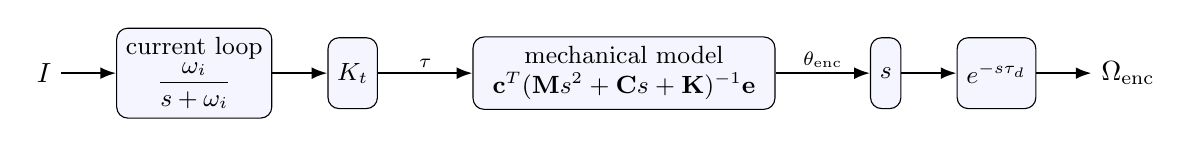
\begin{tikzpicture}[node distance=7mm]
\node (i) {$I$};
\node[blk, right=of i] (cl) {current loop\\ $\dfrac{\omega_i}{s+\omega_i}$};
\node[blk, right=of cl] (kt) {$K_t$};
\node[blk, right=12mm of kt, text width=3.6cm] (mech) {mechanical model\\ $\mathbf c^T(\mathbf Ms^2+\mathbf Cs+\mathbf K)^{-1}\mathbf e$};
\node[blk, right=12mm of mech] (der) {$s$};
\node[blk, right=of der] (del) {$e^{-s\tau_d}$};
\node[right=of del] (o) {$\Omega_\mathrm{enc}$};
\draw[sig] (i) -- (cl); \draw[sig] (cl) -- (kt); \draw[sig] (kt) -- node[above, lab]{$\tau$} (mech);
\draw[sig] (mech) -- node[above, lab]{$\theta_\mathrm{enc}$} (der); \draw[sig] (der) -- (del); \draw[sig] (del) -- (o);
\end{tikzpicture}
\caption{Plant measured by WorkBench (``Plant'' trace) as modelled in~\eqref{eq:plant}. The mechanical block is the elevation model of Figure~\ref{fig:elev} or the azimuth model of Figure~\ref{fig:az}.}\label{fig:plant}
\end{figure}

\subsection{Elevation: H7 with modal masses on the motor stator}\label{sec:elev}
\paragraph{Rotor chain (H7).} The elevation block of H7 has five nodes: encoder disc $e$, hub centre $h$, motor rotor $m$, rear end of the shaft (rear), telescope $p$ (Figure~\ref{fig:elev}).
\begin{itemize}
\item Their inertias are fixed at the CAD/H7 values. The rigid inertia of the axis is $J=\Jaxis$\,kg\,m$^2$.
\item The shaft stiffnesses and dampers $k_{\theta1},c_{\theta1}$ ($e$--$h$), $k_{\theta2},c_{\theta2}$ ($h$--$m$) and $k_{\theta3},c_{\theta3}$ ($m$--rear) are also those of H7.
\item The joint between the telescope and the hub, $k_b$ and $c_b$, is fitted.
\end{itemize}
\paragraph{Stator masses.} Each mode of the fork excited by the stator is a modal oscillator with coordinate $q_r$:
\begin{itemize}
\item it has modal inertia $J_r$, modal stiffness $k_r$ and modal damping $c_r$, all positive, with respect to the ground;
\item the stator reaction $-\tau$ acts on all of them with unit participation;
\item the rotation of the stator structure is the modal superposition $\varphi_s=\sum_r q_r$.
\end{itemize}
\paragraph{Bearings.} The polar bearings are mounted on the same structure. Their pre-sliding friction is a hysteretic spring $k_g^*=k_g(1+j\eta_g)$ between the hub and the stator structure, not the ground.
\paragraph{Encoder.} The disc turns with $\theta_e$, while the read head is carried by the structure and moves by $\sum_r\kappa_r q_r$. The encoder therefore reads
\begin{equation}
\theta_\mathrm{enc}=\theta_e-\sum_{r=1}^{N}\kappa_r q_r .\label{eq:encoder}
\end{equation}
$\kappa_r$ is the rotation of the head per unit of modal coordinate, a kinematic factor and not a stiffness. A negative $\kappa_r$ means that in mode $r$ the head turns against the point where the stator reaction is applied: the motor and the sensor are not collocated for that mode.

\begin{figure}[H]\centering
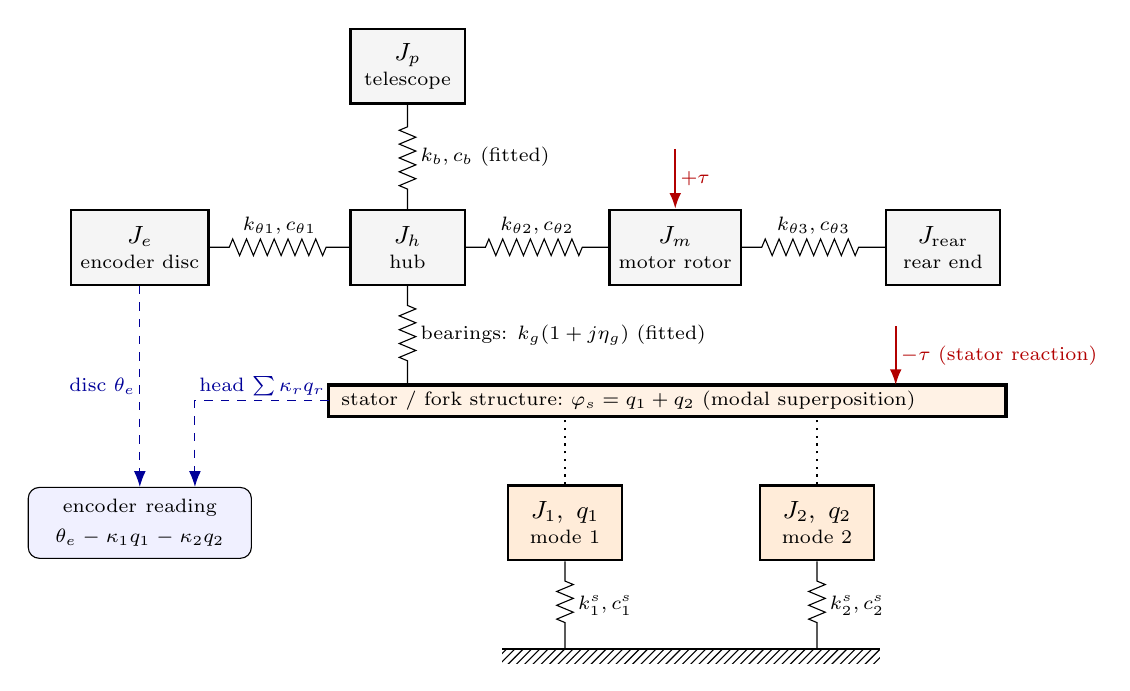
\begin{tikzpicture}[x=1cm, y=1cm]
% rotor chain
\node[mass] (e) at (0,0) {$J_e$\\[-2pt]\scriptsize encoder disc};
\node[mass] (h) at (3.4,0) {$J_h$\\[-2pt]\scriptsize hub};
\node[mass] (m) at (6.8,0) {$J_m$\\[-2pt]\scriptsize motor rotor};
\node[mass] (r) at (10.2,0) {$J_\mathrm{rear}$\\[-2pt]\scriptsize rear end};
\node[mass] (p) at (3.4,2.3) {$J_p$\\[-2pt]\scriptsize telescope};
\draw[spring] (e.east) -- node[above=3pt, lab]{$k_{\theta1},c_{\theta1}$} (h.west);
\draw[spring] (h.east) -- node[above=3pt, lab]{$k_{\theta2},c_{\theta2}$} (m.west);
\draw[spring] (m.east) -- node[above=3pt, lab]{$k_{\theta3},c_{\theta3}$} (r.west);
\draw[spring] (h.north) -- node[right=3pt, lab]{$k_b,c_b$ (fitted)} (p.south);
\draw[sig, red!70!black] (6.8,1.25) -- node[right, lab, red!70!black]{$+\tau$} (m.north);
% stator structure
\draw[very thick, fill=orange!10] (2.4,-2.15) rectangle (11.0,-1.75);
\node[lab, anchor=west] at (2.5,-1.95) {stator / fork structure:\ $\varphi_s=q_1+q_2$ (modal superposition)};
\draw[spring] (h.south) -- node[right=3pt, lab]{bearings: $k_g(1+j\eta_g)$ (fitted)} (3.4,-1.75);
\draw[sig, red!70!black] (9.6,-1.0) -- node[right, lab, red!70!black]{$-\tau$ (stator reaction)} (9.6,-1.75);
% modal masses
\node[mass, fill=orange!15] (q1) at (5.4,-3.5) {$J_1,\ q_1$\\[-2pt]\scriptsize mode 1};
\node[mass, fill=orange!15] (q2) at (8.6,-3.5) {$J_2,\ q_2$\\[-2pt]\scriptsize mode 2};
\draw[dotted, thick] (q1.north) -- (5.4,-2.15); \draw[dotted, thick] (q2.north) -- (8.6,-2.15);
\draw[spring] (q1.south) -- node[right=3pt, lab]{$k_1^s,c_1^s$} (5.4,-5.1);
\draw[spring] (q2.south) -- node[right=3pt, lab]{$k_2^s,c_2^s$} (8.6,-5.1);
\ground{4.6}{9.4}{-5.1}
% encoder reading
\node[blk, fill=blue!6, text width=2.6cm] (enc) at (0,-3.5) {\scriptsize encoder reading\\ $\theta_e-\kappa_1q_1-\kappa_2q_2$};
\draw[meas] (e.south) -- node[left, lab]{disc $\theta_e$} (enc.north);
\draw[meas] (2.4,-1.95) -| node[pos=0.25, above, lab]{head $\sum\kappa_r q_r$} ($(enc.north)+(0.7,0)$);
\end{tikzpicture}
\caption{Elevation model, drawn as its translational analogue (each spring is a spring and a viscous damper in parallel). Grey: rotor chain of H7. Orange: stator structure and its modal oscillators, each grounded by $k_r^s=J_r\omega_r^2$ and $c_r^s=2\zeta_rJ_r\omega_r$. The motor torque acts on the rotor ($+\tau$) and its reaction on the stator ($-\tau$). The bearings join the hub to the stator structure. The encoder reads the disc minus the motion of the head carried by the structure.}\label{fig:elev}
\end{figure}

\paragraph{Equations.} With $\mathbf x=[\theta_e,\theta_h,\theta_m,\theta_\mathrm{rear},\theta_p,q_1,\dots,q_N]^T$, the modal oscillators obey
\begin{equation}
J_r\ddot q_r+c_r^s\dot q_r+k_r^s q_r=-\tau+k_g^*\Bigl(\theta_h-\sum_{s=1}^{N}q_s\Bigr),\qquad k_r^s=J_r\omega_r^2,\quad c_r^s=2\zeta_rJ_r\omega_r ,\label{eq:modal}
\end{equation}
and the hub receives the opposite bearing torque $-k_g^*(\theta_h-\sum_s q_s)$. In the form~\eqref{eq:lumped},
\begin{gather}
\mathbf M=\begin{bmatrix}\mathbf M_0&\\&\mathrm{diag}(J_r)\end{bmatrix},\quad
\mathbf C=\begin{bmatrix}\mathbf C_0(c_b)&\\&\mathrm{diag}(c_r^s)\end{bmatrix},\quad
\mathbf K=\begin{bmatrix}\mathbf K_0(k_b)&\\&\mathrm{diag}(k_r^s)\end{bmatrix}+k_g^*\,\mathbf v\mathbf v^T,\\
\mathbf v=\mathbf e_h-\sum_r\mathbf e_{q_r},\qquad \mathbf e=\mathbf e_m-\sum_r\mathbf e_{q_r},\qquad \mathbf c=\mathbf e_e-\sum_r\kappa_r\,\mathbf e_{q_r},
\end{gather}
where $\mathbf M_0,\mathbf C_0,\mathbf K_0$ are the elevation block of H7 with its $k_b,c_b$ replaced by the fitted ones, and $\mathbf e_j$ is the unit vector of coordinate $j$.

\paragraph{What the measurement can determine.} Neglecting the bearing coupling ($k_g\ll k_r^s$: here \kg\ against $\geq10^5$\,N\,m/rad), mode $r$ adds to $G_\theta$ the term
\begin{equation}
-\kappa_r\frac{q_r}{\tau}=\frac{\kappa_r/J_r}{s^2+2\zeta_r\omega_rs+\omega_r^2}=\frac{a_r}{s^2+2\zeta_r\omega_rs+\omega_r^2},\qquad a_r=\frac{\kappa_r}{J_r} .\label{eq:residue}
\end{equation}
The measurement fixes the modal residue $a_r$, not $J_r$ and $\kappa_r$ separately. The fit therefore estimates $(f_r,\zeta_r,a_r)$ for each mass, and the scale is set by the convention $|\kappa_r|=1$, i.e.\ $J_r=1/|a_r|$ and $\kappa_r=\mathrm{sign}(a_r)$. The $J_r$ of the tables are modal inertias under that convention, not physical inertias of parts.

\subsection{Sign of the residue and non-minimum-phase zeros}\label{sec:nmp}
Above a few hertz the telescope moves with the hub (Section~\ref{sec:res_elev}), and the rotor behaves as the rigid inertia $J$. With the two masses, undamped,
\begin{equation}
G_\theta(s)\simeq\frac{1}{Js^2}+\frac{a_1}{s^2+\omega_1^2}+\frac{a_2}{s^2+\omega_2^2}
=\frac{A u^2+Bu+C}{s^2(s^2+\omega_1^2)(s^2+\omega_2^2)},\qquad u=s^2,
\end{equation}
\begin{equation}
A=\frac1J+a_1+a_2,\qquad B=\frac{\omega_1^2+\omega_2^2}{J}+a_1\omega_2^2+a_2\omega_1^2,\qquad C=\frac{\omega_1^2\omega_2^2}{J} .
\end{equation}
\begin{itemize}
\item \textbf{Positive residues} (collocated actuator and sensor). The zeros interlace with the poles on the imaginary axis ($u$ real and negative): every resonance is preceded by an antiresonance, and the phase comes back after each pair.
\item \textbf{The fitted values} ($J=\Jaxis$\,kg\,m$^2$, $a_1=\aMassI$, $a_2=\aMassII$\,(kg\,m$^2$)$^{-1}$) give $A=\nmpA$, $B=$\,\nmpB\ and $C=$\,\nmpC, so $B^2-4AC=$\,\nmpDisc\,$<0$.
  \begin{itemize}
  \item The two roots $u$ are complex, and the four zeros $s=\pm\sqrt u$ form a quartet $\pm\sigma\pm j\omega$: one pair lies in the right half-plane.
  \item In this approximation the quartet has $|s|/2\pi=\nmpF$\,Hz and $\zeta=\pm\nmpZeta$.
  \item The full model gives \zerosP\ (Figure~\ref{fig:roots}).
  \end{itemize}
\item \textbf{Effect on the phase.} The quartet contributes $+180-180=0^\circ$ instead of the $+360^\circ$ of two collocated antiresonances. Across the two modes the phase therefore falls by $3\times180^\circ$, against $180^\circ$ for a collocated pattern.
\end{itemize}
This is the drop measured between 45 and 120\,Hz, which a model with positive residues only cannot reproduce: a fit restricted to $\kappa_r>0$ ended in a poor local minimum.

\subsection{Azimuth: flexible load}\label{sec:azmodel}
In H7 the azimuth load (fork, hub and ring, $J_\mathrm{load}=\JLcad$\,kg\,m$^2$ from CAD) is one rigid node $L$, with the telescope $P$ attached to it. Here it is split into a fork base $L$ and a fork top $A$ (Figure~\ref{fig:az}):
\begin{equation}
J_L=(1-\alpha)\,J_\mathrm{load},\qquad J_A=\alpha\,J_\mathrm{load},
\end{equation}
\begin{itemize}
\item the two parts are joined by $k_{LA},c_{LA}$, and the total inertia stays the CAD value;
\item the telescope hangs from the fork top through $k_3,c_3$;
\item the bearing constraint $k_g(1+j\eta_g)$ grounds the fork base;
\item the motor shaft $k_2,c_2$ is fitted, while the encoder shaft $k_1=\kone$\,N\,m/rad and the inertias $J_e,J_m,J_P$ are those of H7.
\end{itemize}
With $\mathbf x=[\psi_e,\psi_m,\psi_L,\psi_A,\psi_P]^T$, the model~\eqref{eq:lumped} has $\mathbf M=\mathrm{diag}(J_e,J_m,J_L,J_A,J_P)$ and a chain $\mathbf K$, $\mathbf C$ of the four links, with $k_g^*$ added at $(L,L)$; $\mathbf e=\mathbf e_m$ and $\mathbf c=\mathbf e_e$.

\begin{figure}[H]\centering
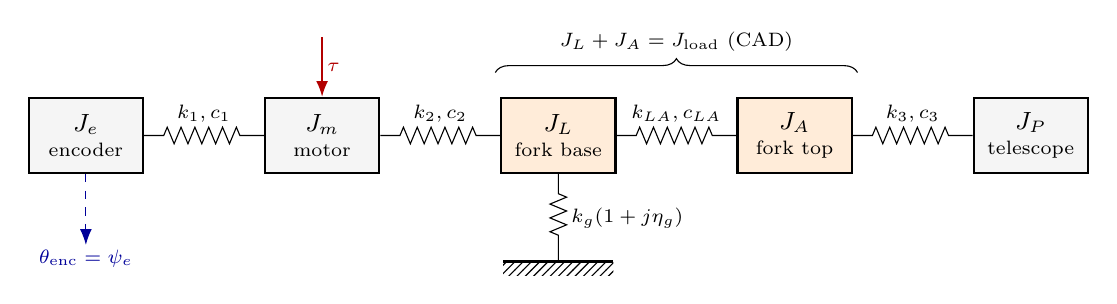
\begin{tikzpicture}[x=1cm, y=1cm]
\node[mass] (e) at (0,0) {$J_e$\\[-2pt]\scriptsize encoder};
\node[mass] (m) at (3.0,0) {$J_m$\\[-2pt]\scriptsize motor};
\node[mass, fill=orange!15] (L) at (6.0,0) {$J_L$\\[-2pt]\scriptsize fork base};
\node[mass, fill=orange!15] (A) at (9.0,0) {$J_A$\\[-2pt]\scriptsize fork top};
\node[mass] (P) at (12.0,0) {$J_P$\\[-2pt]\scriptsize telescope};
\draw[spring] (e.east) -- node[above=3pt, lab]{$k_1,c_1$} (m.west);
\draw[spring] (m.east) -- node[above=3pt, lab]{$k_2,c_2$} (L.west);
\draw[spring] (L.east) -- node[above=3pt, lab]{$k_{LA},c_{LA}$} (A.west);
\draw[spring] (A.east) -- node[above=3pt, lab]{$k_3,c_3$} (P.west);
\draw[spring] (L.south) -- node[right=3pt, lab]{$k_g(1+j\eta_g)$} (6.0,-1.6);
\ground{5.3}{6.7}{-1.6}
\draw[sig, red!70!black] (3.0,1.25) -- node[right, lab, red!70!black]{$\tau$} (m.north);
\draw[meas] (e.south) -- ++(0,-0.9) node[below, lab]{$\theta_\mathrm{enc}=\psi_e$};
\draw[decorate, decoration={brace, amplitude=5pt}] (5.2,0.8) -- node[above=6pt, lab, align=center]{$J_L+J_A=J_\mathrm{load}$ (CAD)} (9.8,0.8);
\end{tikzpicture}
\caption{Azimuth model with the flexible load, drawn as its translational analogue (each spring is a spring and a viscous damper in parallel). Orange: the H7 load node split into fork base and fork top.}\label{fig:az}
\end{figure}

%% ===================================================================================================
\section{Identification}\label{sec:method}
\begin{figure}[H]\centering
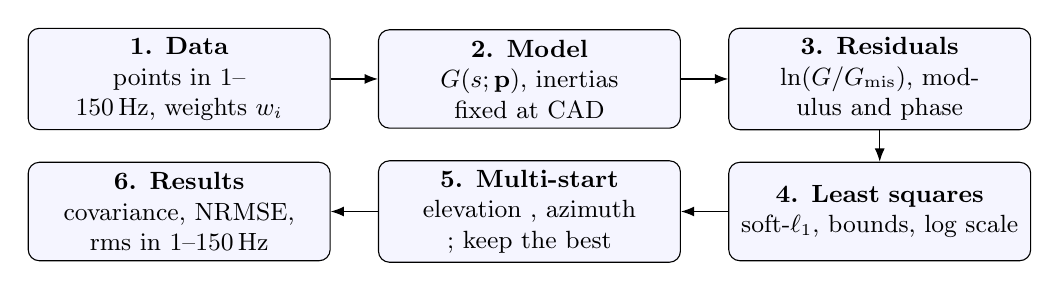
\begin{tikzpicture}[node distance=4mm and 6mm, every node/.style={font=\small},
  box/.style={draw, rounded corners, align=center, text width=3.6cm, minimum height=1.25cm, fill=blue!4}]
\node[box] (a) {\textbf{1. Data}\\ points in 1--150\,Hz, weights $w_i$};
\node[box, right=of a] (b) {\textbf{2. Model}\\ $G(s;\mathbf p)$, inertias fixed at CAD};
\node[box, right=of b] (c) {\textbf{3. Residuals}\\ $\ln(G/G_\mathrm{mis})$, modulus and phase};
\node[box, below=of c] (d) {\textbf{4. Least squares}\\ soft-$\ell_1$, bounds, log scale};
\node[box, left=of d] (e) {\textbf{5. Multi-start}\\ elevation \nStartsP, azimuth \nStartsA; keep the best};
\node[box, left=of e] (f) {\textbf{6. Results}\\ covariance, NRMSE, rms in 1--150\,Hz};
\draw[-{Latex}] (a) -- (b); \draw[-{Latex}] (b) -- (c); \draw[-{Latex}] (c) -- (d); \draw[-{Latex}] (d) -- (e); \draw[-{Latex}] (e) -- (f);
\end{tikzpicture}
\caption{Flow of the identification, run separately for the two axes by \texttt{analisi\_modi\_forcella.py} (model in \texttt{src/gimbal\_mdof/modi\_forcella.py}).}\label{fig:flow}
\end{figure}

\subsection{Error and cost}
\paragraph{Error.} At each measured frequency $f_i$ the error is the complex logarithm of the ratio of model to measurement:
\begin{equation}
\varepsilon_i=\ln\frac{G(j\omega_i;\mathbf p)}{G_\mathrm{mis}(j\omega_i)}=\underbrace{\ln\left|\frac{G}{G_\mathrm{mis}}\right|}_{\text{magnitude, Np}}+j\,\underbrace{\bigl(\angle G-\angle G_\mathrm{mis}\bigr)}_{\text{phase, rad}} .
\end{equation}
\begin{itemize}
\item Magnitude and phase weigh alike: 1\,Np = 8.7\,dB counts as 1\,rad = 57.3$^\circ$.
\item The phase difference is taken on the ratio, so it does not depend on the unwrapping.
\item Antiresonances (small $|G|$) count as much as resonances, unlike an error on $G$ itself.
\end{itemize}

\paragraph{Weights.} The grids differ (1 to 3\,\% steps) and the three elevation measurements overlap. Each point is weighted by the width of the frequency interval it represents:
\begin{equation}
w_i=\sqrt{\frac{\Delta\ln f_i}{0.01}},
\end{equation}
so that the cost is an integral over $\ln f$, and a finer grid does not weigh more than a coarser one over the same band. The residual vector is $\mathbf r=[\,w_i\,\mathrm{Re}\,\varepsilon_i,\ w_i\,\mathrm{Im}\,\varepsilon_i\,]$ over all the points of all the measurements of the axis.

\paragraph{Cost.} A robust soft-$\ell_1$ loss limits the weight of the points the model cannot follow (the 8--9\,Hz pair, the small features at 48--50 and 84\,Hz):
\begin{equation}
F(\mathbf p)=\frac12\sum_j C^2\rho\!\left(\frac{r_j^2}{C^2}\right),\qquad \rho(z)=2\bigl(\sqrt{1+z}-1\bigr),\qquad C=\lossScale ,
\end{equation}
quadratic for $|r_j|\ll C$ (0.1\,Np $\approx$ 0.9\,dB, 0.1\,rad $\approx$ 5.7$^\circ$) and linear above.

\subsection{Parameters, bounds and starts}
\begin{itemize}
\item \textbf{Scale.} The positive parameters are fitted on their logarithm (relative steps, positivity). The residues $a_r$, which carry a sign, are fitted on their value.
\item \textbf{Elevation.}
  \begin{itemize}
  \item Fitted: $k_b$, $c_b$, $k_g$, $\eta_g$, $\tau_d$, and $(f_r,\zeta_r,a_r)$ of each mass.
  \item Bounds on $f_r$: $\pm10\,\%$ of the start (58.5 and 99.2\,Hz, the measured resonances). Bounds on $a_r$: $[-50,50]$.
  \item \nStartsP\ starts: $k_b\in\{\kbHseven,10^6\}$\,N\,m/rad, both signs of each residue, and $|a_r|\in\{0.3,1.5\}$, below and above $1/J=\invJaxis$.
  \end{itemize}
\item \textbf{Azimuth.}
  \begin{itemize}
  \item Fitted: $\alpha$, $k_{LA}$, $c_{LA}$, $k_3$, $c_3$, $k_2$, $c_2$, $k_g$, $\eta_g$, $\tau_d$.
  \item \nStartsA\ starts: $\alpha\in\{0.2,0.4,0.7\}$ combined with three assignments of the measured 49 and 56\,Hz resonances to the base--top link and to the telescope: (49, 56), (56, 49), and (56\,Hz, telescope stiff at 120\,Hz).
  \end{itemize}
\item \textbf{Solver.} Trust-region reflective least squares (\texttt{scipy.optimize.least\_squares}, Jacobian scaling), at most 800 evaluations per start. The start with the lowest cost is kept.
\end{itemize}
The bounds and the starts of every parameter are in Tables~\ref{tab:polar_params} and~\ref{tab:az_params}.

\subsection{Uncertainty and goodness measures}
\paragraph{Uncertainty.} From the Jacobian $\mathbf J$ of the residuals at the optimum,
\begin{equation}
\mathrm{cov}(\mathbf x)=s^2\,(\mathbf J^T\mathbf J)^{+},\qquad s^2=\frac{2F}{m-n},
\end{equation}
with $m$ residuals and $n$ parameters. For a parameter fitted on its logarithm, the standard deviation of $\ln p$ is its relative standard deviation. A value above 100\,\% means that the data do not determine the parameter.

\paragraph{Fit.} The NRMSE fit of the System Identification Toolbox, on the complex response at the measured points of a band:
\begin{equation}
\mathrm{fit}=100\left(1-\frac{\lVert G_\mathrm{mis}-G\rVert}{\lVert G_\mathrm{mis}-\overline{G_\mathrm{mis}}\rVert}\right)\ \% .
\end{equation}
\begin{itemize}
\item It is reported over the whole fit band (1--150\,Hz) and in the sub-bands 1--5, 5--100 and 100--150\,Hz.
\item On the complex response it is dominated by the points of large magnitude (resonances, low frequency).
\item The rms of $20\log_{10}|G/G_\mathrm{mis}|$ (dB) and of the phase error (deg) weigh all the points alike.
\end{itemize}

%% ===================================================================================================
\section{Results: elevation}\label{sec:res_elev}
\paragraph{Convergence.} All \nStartsP\ starts end at the same cost, \costP. The minimum does not depend on the signs or moduli of the starting residues. The best start places a negative residue on the mass at \fMassI\,Hz and a positive one on the mass at \fMassII\,Hz.

\begin{table}[H]\centering\small
\caption{Elevation: fitted parameters. H7: value in the configuration. Start: values of the \nStartsP\ starts. Std: relative standard deviation from the Jacobian.}\label{tab:polar_params}
\begin{tabular}{llrrL{3.0cm}lrl}\toprule
parameter & unit & estimate & H7 & start & bounds & std & at bound \\ \midrule
\input{generated/tab_polar_params}\\ \bottomrule
\end{tabular}\end{table}

\begin{table}[H]\centering\small
\caption{Elevation: stator masses. $J_r=1/|a_r|$ and $\kappa_r=\mathrm{sign}(a_r)$ under the convention $|\kappa_r|=1$; $k_r^s=J_r\omega_r^2$, $c_r^s=2\zeta_rJ_r\omega_r$.}\label{tab:masses}
\begin{tabular}{lrrrrrrr}\toprule
mass & $f_r$ [Hz] & $\zeta_r$ & $a_r$ [1/(kg\,m$^2$)] & $J_r$ [kg\,m$^2$] & $\kappa_r$ & $k_r^s$ [N\,m/rad] & $c_r^s$ [N\,m\,s/rad] \\ \midrule
\input{generated/tab_masses}\\ \bottomrule
\end{tabular}\end{table}

\paragraph{Stator masses.}
\begin{itemize}
\item \textbf{Mass 1} ($f_1=\fMassI$\,Hz, $\zeta_1=\zMassI$, $a_1=\aMassI$). It takes up the measured pair of resonances at 56.3 and 58.5\,Hz as a single mode: the model peak (57.6\,Hz) falls between the two measured ones.
  \begin{itemize}
  \item Its negative residue makes it non-collocated (Section~\ref{sec:nmp}).
  \item $a_1J=\aOneJ$: its residue is 63\,\% of the rotor one, $1/J$, with the opposite sign, which is large enough to produce the right-half-plane zeros.
  \end{itemize}
\item \textbf{Mass 2} ($f_2=\fMassII$\,Hz, $\zeta_2=\zMassII$, $a_2=\aMassII$) is collocated.
\item Frequencies, damping ratios and residues are determined within 6\,\%.
\end{itemize}

\paragraph{Telescope joint.} $k_b$ goes to its lower bound and is not determined, while $c_b=\cb$\,N\,m\,s/rad. The joint acts as a damper that couples the telescope to the hub up to $c_b/J_p\approx2\pi\cdot400$\,Hz. Below 150\,Hz the data only require that the telescope moves with the hub, and the antiresonance of H7 at 58\,Hz (from $k_b=\kbHseven$\,N\,m/rad) is not seen. The four-mass fit reached the same conclusion with a different pair ($k_b=8\times10^5$\,N\,m/rad, $c_b=717$\,N\,m\,s/rad).

\paragraph{Bearings and delay.}
\begin{itemize}
\item $k_g=\kg$\,N\,m/rad, $\eta_g=\etag$, close to the ground constraint of the configuration (164\,N\,m/rad, 3.11). They set the low-frequency rigid-body pole at 1.8\,Hz.
\item The same model with the bearings to the ground instead of to the stator gives the same cost (\costPground\ against \costP). With two masses the data cannot tell where the bearings are attached.
\item The equivalent delay is $\tau_d=\taudP$\,ms.
\end{itemize}

\begin{figure}[H]\centering
\includegraphics[width=\linewidth]{figures/polar_bode.pdf}
\caption{Elevation plant [dB (rad/s)/A] and phase [deg] in the fit band: the three measurements and the model with two stator masses. Right: zoom 40--150\,Hz.}\label{fig:polar_bode}
\end{figure}

\paragraph{Decomposition of the encoder reading} (Figure~\ref{fig:contrib}).
\begin{itemize}
\item The rotor term $\theta_e$ carries the whole response up to about 40\,Hz.
\item Mass 1 dominates around 57\,Hz.
\item Between 60 and 90\,Hz, the term of mass 1 (phase near $+90^\circ$, Figure~\ref{fig:contrib}) and the term of mass 2 partly cancel the rotor term. This is where the non-minimum-phase quartet lies.
\item Mass 2 dominates around 100\,Hz.
\end{itemize}

\begin{figure}[H]\centering
\includegraphics[width=0.92\linewidth]{figures/polar_contributions.pdf}
\caption{Elevation model: encoder reading~\eqref{eq:encoder} [dB (rad/s)/A, deg] split into the encoder disc term (rotor) and the head motion of each stator mass, $-\kappa_rq_r$, each with the plant factors of~\eqref{eq:plant}. Grey dots: 1--600\,Hz measurement in the band.}\label{fig:contrib}
\end{figure}

\begin{figure}[H]\centering
\includegraphics[width=0.9\linewidth]{figures/roots.pdf}
\caption{Poles (crosses) and zeros (circles) of $G_\theta$ below 150\,Hz, upper half of the $s$-plane, in Hz, with the damping ratio. Shaded: right half-plane. Elevation: the zero at 74.6\,Hz with $\zeta<0$ and its mirror image at 81.8\,Hz form the quartet of Section~\ref{sec:nmp}.}\label{fig:roots}
\end{figure}

%% ===================================================================================================
\section{Results: azimuth}\label{sec:res_az}
\begin{table}[H]\centering\footnotesize
\caption{Azimuth: fitted parameters. H7: value in the configuration. Start: values of the \nStartsA\ starts. Std: relative standard deviation from the Jacobian.}\label{tab:az_params}
\setlength{\tabcolsep}{4pt}\begin{tabular}{llrrL{3.2cm}lrl}\toprule
parameter & unit & estimate & H7 & start & bounds & std & at bound \\ \midrule
\input{generated/tab_azimuth_params}\\ \bottomrule
\end{tabular}\end{table}

\paragraph{Load split.} The fork top takes $\alpha=\alphaA$ of the CAD load:
\begin{itemize}
\item $J_A=\JA$\,kg\,m$^2$ for the fork top and $J_L=\JL$\,kg\,m$^2$ for the fork base;
\item the base--top link has $k_{LA}=$\,\kLA\,N\,m/rad;
\item the motor shaft comes out stiffer than in H7, $k_2=$\,\ktwo\ against \ktwoHseven\,N\,m/rad.
\end{itemize}
Two dampers, $c_{LA}$ and $c_2$, go to their lower bound and are not determined: the damping of the fork mode is supplied by $c_3$.

\paragraph{Modes} (Table~\ref{tab:az_modes}).
\begin{itemize}
\item The rigid-body mode on the bearing constraint is at \fRigidAz\,Hz.
\item The fork mode is at \fForkAz\,Hz, with $\zeta=\zForkAz$. In it the encoder, the motor and the fork base move together against the fork top and the telescope.
\item This mode gives the measured antiresonance--resonance--antiresonance pattern: 12.3/55.7/64.6\,Hz measured, 12.9/54.8/64.0\,Hz in the model (Table~\ref{tab:features}).
\end{itemize}

\begin{table}[H]\centering\small
\caption{Azimuth: modes of the fitted model below 150\,Hz (real stiffness of the constraint), shapes normalised on the largest node.}\label{tab:az_modes}
\begin{tabular}{lrrrrrrr}\toprule
mode & $f$ [Hz] & $\zeta$ & $e$ & $m$ & $L$ & $A$ & $P$ \\ \midrule
\input{generated/tab_azimuth_modes}\\ \bottomrule
\end{tabular}\end{table}

\paragraph{Telescope joint and second minimum.} The best fit gives $k_3=$\,\kthree\,N\,m/rad with $c_3=\cthree$\,N\,m\,s/rad. This is an overdamped telescope, $\zeta\approx c_3/(2\sqrt{k_3J_P})\approx0.9$, with a standard deviation of 22\,\% on $k_3$ and 63\,\% on $c_3$. The \nStartsA\ starts end in three minima, with costs \costsA:
\begin{itemize}
\item The second (+10\,\%) keeps the telescope joint near its H7 value: $k_3=1.18\times10^5$\,N\,m/rad, $c_3=22.6$\,N\,m\,s/rad, $\alpha=0.726$.
\item It adds a lightly damped telescope mode at 86.8\,Hz ($\zeta=0.059$) that the measurement does not show clearly.
\item The data in the band discriminate only weakly between the two descriptions of the telescope.
\end{itemize}

\paragraph{Bearings and delay.} $k_g=\kgA$\,N\,m/rad and $\eta_g=\etaA$; the ground constraint of the configuration is 1418\,N\,m/rad and 0.32. The delay $\tau_d=\taudA$\,ms is poorly determined (84\,\%).

\begin{figure}[H]\centering
\includegraphics[width=\linewidth]{figures/azimuth_bode.pdf}
\caption{Azimuth plant [dB (rad/s)/A] and phase [deg] in the fit band: measurement and model with the flexible load. Right: zoom 40--150\,Hz.}\label{fig:az_bode}
\end{figure}

\paragraph{Consistency between the axes.} The fork mode seen by the azimuth encoder (\fForkAz\,Hz) and the elevation stator mass 1 (\fMassI\,Hz) are within 2\,Hz. This agrees with the hypothesis that the resonances near 56\,Hz on both axes are the same vibration of the fork. The two axes are still fitted separately: the frequencies are not shared parameters.

%% ===================================================================================================
\section{Fit quality in the band 1--150\,Hz}\label{sec:quality}
\begin{table}[H]\centering\footnotesize
\caption{Fit (NRMSE, \%) on the measured points in the fit band and in its sub-bands, and rms errors over the band. ``--'': no points in the sub-band. H7: the configuration, not fitted.}\label{tab:fit}
\setlength{\tabcolsep}{4pt}\begin{tabular}{lL{2.3cm}L{4.6cm}rrrrrr}\toprule
axis & model & measurement & 1--150 & 1--5 & 5--100 & 100--150 & rms [dB] & rms [deg] \\ \midrule
\input{generated/tab_fit}\\ \bottomrule
\end{tabular}\end{table}

\begin{figure}[H]\centering
\includegraphics[width=0.92\linewidth]{figures/fit_errors.pdf}
\caption{Error of the fitted models on each measurement in the fit band: magnitude [dB] and phase [deg], $\varepsilon_i$ converted from Np and rad.}\label{fig:errors}
\end{figure}

\paragraph{Where the models miss} (Figures~\ref{fig:polar_bode}, \ref{fig:az_bode} and~\ref{fig:errors}).
\begin{itemize}
\item \textbf{Elevation, 7--10\,Hz.} The measured antiresonance at 8.1\,Hz and resonance at 9\,Hz are not in the model: up to 8\,dB and 80$^\circ$ of error. This is the price of removing the mass at 8.8\,Hz, and it explains the 32\,\% of the 1--600\,Hz measurement between 5 and 100\,Hz.
\item \textbf{Elevation, 40--55\,Hz.} The measured small antiresonance at 48--51\,Hz is not modelled, and the model lies 1--2\,dB above the measurement before the peak. The mass at 53.4\,Hz of the four-mass model covered this region.
\item \textbf{Elevation, 56--59\,Hz.} The measured double peak (56.3 and 58.5\,Hz) is one peak at 57.6\,Hz in the model.
\item \textbf{Elevation, 84\,Hz.} The small measured feature is not modelled.
\item \textbf{Azimuth, 48--50\,Hz.} The small measured pair of features is not modelled.
\end{itemize}

\begin{table}[H]\centering\small
\caption{Measured and modelled antiresonances and resonances in the fit band (peaks of at least 3\,dB prominence).}\label{tab:features}
\begin{tabular}{L{6.4cm}ll}\toprule
curve & antiresonances [Hz] & resonances [Hz] \\ \midrule
\input{generated/tab_features}\\ \bottomrule
\end{tabular}\end{table}

\paragraph{Two masses against four.} Table~\ref{tab:compare} compares the reported model with the previous four-mass one (masses at \massesFour\,Hz), fitted on the same data and band.
\begin{itemize}
\item The total elevation cost rises from \costPfour\ to \costP, almost all of it on the 1--600\,Hz measurement below 50\,Hz.
\item On the two measurements that start at 30\,Hz, the two-mass model is slightly better. Without the low-frequency masses, the robust cost spends its effort on the fork modes.
\end{itemize}

\begin{table}[H]\centering\small
\caption{Elevation: fit (NRMSE, \%) of the four-mass (4m) and of the two-mass (2m) models in the fit band and its sub-bands, and rms phase error [deg].}\label{tab:compare}
\begin{tabular}{L{4.2cm}rrrrrrrrrr}\toprule
& \multicolumn{2}{c}{1--150\,Hz} & \multicolumn{2}{c}{1--5\,Hz} & \multicolumn{2}{c}{5--100\,Hz} & \multicolumn{2}{c}{100--150\,Hz} & \multicolumn{2}{c}{rms [deg]} \\
\cmidrule(lr){2-3}\cmidrule(lr){4-5}\cmidrule(lr){6-7}\cmidrule(lr){8-9}\cmidrule(lr){10-11}
measurement & 4m & 2m & 4m & 2m & 4m & 2m & 4m & 2m & 4m & 2m \\ \midrule
\input{generated/tab_compare}\\ \bottomrule
\end{tabular}\end{table}

%% ===================================================================================================
\section{Limitations and open points}\label{sec:limits}
\begin{itemize}
\item \textbf{Modal inertias.} Only $a_r=\kappa_r/J_r$ is identifiable. A physical modal inertia would need the motion of the stator measured independently, for example with an accelerometer on the fork.
\item \textbf{Low frequency.} The elevation pair at 8--9\,Hz is left out by choice. If the loop design needs it, the mass at about 9\,Hz can be put back (three masses).
  \begin{itemize}
  \item Its sharp antiresonance and damped resonance were reproduced only with an equivalent damping ratio of 0.17.
  \item This suggests a friction-related, amplitude-dependent mechanism.
  \end{itemize}
\item \textbf{Telescope joints.} Neither $k_b$ (elevation) nor $k_3$, $c_3$ (azimuth) are determined in the band. Both data sets only require the telescope to follow its support up to 150\,Hz.
\item \textbf{Dampers of the azimuth chain.} $c_{LA}$ and $c_2$ are at their lower bound, and the azimuth delay is not determined.
\item \textbf{Linear model.} The bearing constraint is a linear hysteretic equivalent fitted at the amplitude of these tests (3--4\,A); it does not hold for other amplitudes.
\item \textbf{Separate fits.} The two axes are fitted separately. A joint fit with shared fork modes, and the use of the coherence once it is exported, are the natural next steps.
\end{itemize}

\end{document}
